\documentclass[a4paper,11pt,titlepage]{article}
\usepackage{hyperref}
\usepackage[svgnames,dvipsnames]{xcolor}
\usepackage{listings}
\usepackage{caption}
\usepackage{enumitem} % For \begin{itemize}[label=$\star$]
\usepackage{titlepic}
\usepackage{graphicx}

% how to format source code / benchmark names
\newcommand{\sourcecode}[1]{{\tt #1}}
\newcommand{\bm}[1]{{\tt #1}}
\newcommand{\cmd}[1]{{\tt #1}}
\newcommand{\opt}[1]{{\tt #1}}
\newcommand{\ignore}[1]{}

% From http://tex.stackexchange.com/questions/823/remove-ugly-borders-around-clickable-crossreferences-and-hyperlinks
\hypersetup{
    colorlinks=false,
    pdfborder={0 0 0},
}

% From http://tex.stackexchange.com/questions/7526/toc-section-subsection-coloring
% Color listing: http://www.math.washington.edu/tex-archive/macros/latex/contrib/xcolor/xcolor.pdf
\makeatletter
\let\stdl@section\l@section
\renewcommand*{\l@section}[2]{%
  \stdl@section{\textcolor{MidnightBlue}{#1}}{\textcolor{black}{#2}}}
\let\stdl@subsection\l@subsection
\renewcommand*{\l@subsection}[2]{%
  \stdl@subsection{\textcolor{DarkSlateBlue}{#1}}{\textcolor{black}{#2}}}
\makeatother


% From http://tex.stackexchange.com/questions/14967/source-code-listing-with-frame-around-code
\DeclareCaptionFont{white}{\color{white}}
\DeclareCaptionFormat{listing}{%
  \parbox{\textwidth}{\colorbox{DarkSlateBlue}{\parbox{\textwidth}{#1#2#3}}\vskip-4pt}}
\captionsetup[lstlisting]{format=listing,labelfont=white,textfont=white}
\definecolor{dkgreen}{rgb}{0,0.6,0}
\definecolor{gray}{rgb}{0.5,0.5,0.5}
\definecolor{mauve}{rgb}{0.58,0,0.82}
\lstset{
        frame=lrb,
        xleftmargin=\fboxsep,
        xrightmargin=-\fboxsep,
        breaklines=true,
        basicstyle=\footnotesize\ttfamily,
        keywordstyle=\color{BrickRed},
        commentstyle=\color{dkgreen},
        stringstyle=\color{mauve},
        alsoletter={\#,[,],/},
        showstringspaces=false,
       }
\lstdefinelanguage{ini}{
%        keywordsprefix={[},
        morekeywords={/,[,]},
        otherkeywords={\#include},
        morestring=[b]",
        morecomment=[l]{;},
        morecomment=[l]{\#},
       }


\author{Trevor~E.~Carlson \and Wim~Heirman}

\title{The Sniper User Manual}

\titlepic{
\includegraphics[width=.35\textwidth]{sniperlogo.pdf}}

\begin{document}

\maketitle
\setcounter{tocdepth}{2}
\tableofcontents

\section{Introduction}

\subsection{What is Sniper?}

Sniper is a next generation parallel, high-speed and accurate x86 simulator.
This multi-core simulator is based on the interval core model and the
Graphite simulation infrastructure, allowing for fast and accurate simulation
and for trading off simulation speed for accuracy to allow a range of flexible
simulation options when exploring different homogeneous and heterogeneous multi-core architectures.
%Using this methodology, we are able to achieve good accuracy against hardware for 16-thread applications.

The Sniper simulator allows one to perform timing simulations for both multi-programmed workloads
and multi-threaded, shared-memory applications running on 10s to 100+ cores, at a high speed when compared
to existing simulators. The main feature of the simulator is its core model which
is based on interval simulation, a fast mechanistic core model. Interval simulation
raises the level of abstraction in architectural simulation which allows for
faster simulator development and evaluation times; it does so by 'jumping' between
miss events, called intervals.
Sniper has been validated against multi-socket Intel Core2 and Nehalem systems
and provides average performance prediction errors within 25\%
at a simulation speed of up to several MIPS.

This simulator, and the interval core model, is useful for uncore and system-level
studies that require more detail than the typical one-IPC models, but for which cycle-accurate
simulators are too slow to allow workloads of meaningful sizes to be simulated.
As an added benefit,
the interval core model allows the generation of CPI stacks, which show the number
of cycles lost due to different characteristics of the system, like the cache hierarchy
or branch predictor, and lead to a better understanding of each component's
effect on total system performance. This extends the use for Sniper
to application characterization and hardware/software co-design.
The Sniper simulator is available for download at \texttt{\footnotesize{http://snipersim.org}}
and can be used freely for academic research.

%\subsection{What can I do with Sniper?}

%Simulate shared-memory multi-core x86 computers to determine application runtime performance.

\subsection{Features}

  \begin{itemize}
  \item Interval core model
  \item CPI Stack generation
  \item Parallel, multi-threaded simulator
  \item Multi-threaded application support
  \item Multi-program workload support with the SIFT trace format
  \item Validated against the Core2 microarchitecture
  \item Shared and private caches
  \item Heterogeneous core configuration
  \item Modern, Pentium-M style branch predictor
  \item Supports a number of pthread-based parallel application APIs, like OpenMP, TBB and OpenCL
  \item SimAPI and Python interfaces for monitoring and controlling the simulator's behavior at runtime
  \item ROI (region of interest) support
  \item Multiple instrumentation modes - Faster cache-only pre-ROI simulation
  \item Single-option debugging of simulator or application itself
  \item Stackable configurations
  \item x86-64 support and initial 32-bit support
  \item Modern Linux-OS support
  \item Integrated statistics collection support
  \end{itemize}

\section{Getting Started}

\subsection{Downloading Sniper}
\label{sec:download}

Download Sniper at \url{http://www.snipersim.org/w/Download}.

\subsection{Compiling Sniper}

One can compile Sniper with the following command: \sourcecode{cd sniper \&\& make}.  If you have multiple processors, you can take advantage of a parallel make build starting with Sniper version 3.0.  In that case, you can run \sourcecode{make -j N}, where \sourcecode{N} is the number of make processes to start.

The SNIPER\_TARGET\_ARCH environment variable can be use to set the architecture type for compilation. If you are running on a 64-bit host (\cmd{intel64}), then
setting the SNIPER\_TARGET\_ARCH variable to \cmd{ia32} will compile Sniper and the applications in the {sniper/test} in 32-bit mode.

\subsection{Running a Test Application}

After compiling Sniper, you can run the included test application to verify that the simulator
has been compiled properly.

\belowcaptionskip=-10pt
\begin{lstlisting}[label=run-test-app,caption=Running an included application,rulecolor=\color{DarkSlateBlue},language=Bash,deletekeywords=test]
$ cd sniper/test/fft
$ make run
...
[SNIPER] Start
\end{lstlisting}

\section{Running Sniper}

To run Sniper, use the \cmd{run-sniper} command. For more details on all of the options that \cmd{run-sniper}
accepts, see Section~\ref{sec:cmd-run-sniper}.

Here is the most basic example of how to run the Sniper simulator.  After execution, there will be
a number of files created that provide an overview of the current simulation run.

\begin{lstlisting}[label=benchmarks-quickstart,caption=Integrated Benchmarks Quickstart,rulecolor=\color{DarkSlateBlue},language=Bash]
$ cd sniper
$ ./run-sniper -- /bin/ls
\end{lstlisting}

\subsection{Simulation Output}

After running Sniper, output will be created in the current directory (or a directory specified
by the \cmd{-d} option to run-sniper).  With the files created there, one can see the results
of the timing simulation done by Sniper.

The main file generated is the \cmd{sim.out} file.  It is generated automatically by the
\sourcecode{sniper/tools/gen\_simout.py} command, and contains basic information about the simulation,
such as runtime, instruction count, and simulated cycles. (Note that cycle count is only correct
when there has only been a single core frequency during the entire run.)

In addition to viewing the \cmd{sim.out} file, we encourage the use of the \sourcecode{sniper/tools/sniper\_lib.py:get\_results()} function to parse and process results.
The \cmd{sim.stats} files store the raw counter information that
has been recorded by the different components of Sniper.
Since Sniper 4.0, the new SQLite3 statisitics database format (\cmd{sim.stats.sqlite3}) supports
multiple statistics snapshots over time.
No matter which \cmd{sim.stats} data format is in the back end, the \sourcecode{get\_results()}
python subroutine will be able to present a consistent view of the statistics.  Additionally, the
\cmd{sniper/tools/dumpstats.py} utility will continue to produce human-readable output
of all of the counters no matter what the back end will be.

\subsection{Using the Integrated Benchmarks}
\label{sec:integrated-benchmarks}

Download Sniper as described in Section~\ref{sec:download}, and then follow the example in Listing~\ref{benchmarks-quickstart}.

\begin{lstlisting}[label=benchmarks-quickstart,caption=Integrated Benchmarks Quickstart,rulecolor=\color{DarkSlateBlue},language=Bash]
$ wget http://snipersim.org/packages/sniper-benchmarks.tbz
$ tar xjf sniper-benchmarks.tbz
$ cd benchmarks
$ export SNIPER_ROOT=/path/to/sniper
$ export BENCHMARKS_ROOT=$(pwd)
$ make -j 2              # make -j supported in Sniper 3.0
$ ./run-sniper -p splash2-fft -i small -n 4 -c gainestown
\end{lstlisting}

\subsubsection{Automatically Running Multiple Multi-threaded Workloads}

Starting with Sniper version 3.04, and using the integrated benchmarks as described in Section~\ref{sec:integrated-benchmarks},
it is now possible to run multiple multi-threaded workloads in parallel (or easily run multiple multi-program workloads
in parallel). To do this, one needs to simply use the \cmd{--benchmarks} option to \cmd{\$BENCHMARKS\_ROOT/run-sniper}.
Note that currently, ROI support is disabled and the entire application will run in the simulator (not just the region
of interest).

\begin{lstlisting}[label=benchmarks-multiple-multi-threaded,caption=Running Multiple Multi-threaded Benchmarks,rulecolor=\color{DarkSlateBlue},language=Bash]
$ cd $BENCHMARKS_ROOT
$ ./run-sniper -c gainestown --benchmarks=splash2-fft-small-2,splash2-fft-small-2
\end{lstlisting}


\subsection{Simulation modes}

When running a single (potentially multi-threaded) application, Sniper uses the Pin front-end
which supports multiple simulation modes, these can be switched at runtime. These modes are:

\begin{itemize}
\item Detailed --- Fully detailed models of cores, caches and interconnection network
\item Cache-only --- No core model (simulated time does not advance!), only simulate cache hit rates (useful for cache and branch predictor warmup)
\item Fast-forward --- No core and no cache models, useful for quickly skipping to a region of interest
\end{itemize}

As a (rough) guideline, simulation speed is in the order of 1 MIPS (detailed) / 10 MIPS (cache-only)
/ 1000 MIPS (fast-forward) when using the different instrumentation modes.


\subsection{Region of interest (ROI)}

When simulating parallel applications, one usually does not care about the (sequential) initialization
and cleanup phases of the benchmarks. When applications are marked with \opt{SimRoiBegin()} and \opt{SimRoiEnd()}
markers, Sniper can enable performance models only during ROI. By default, Sniper assumes the application
has no such markers and simulates the entire application in detailed mode. The \opt{--roi} option to \cmd{run-sniper}
changes this behavior, and starts in cache-only mode (the initialization phase is used to warm up caches,
the \opt{--no-cache-warming} option can be used to select fast-forward mode instead)
until the application executes \opt{SimRoiBegin()}, and switches to fast-forward mode on \opt{SimRoiEnd()}.
The integrated benchmarks suite already has ROI markers included, in fact, when using the \cmd{run-sniper}
script inside \opt{benchmarks}, \opt{--roi} is implied (use \cmd{benchmarks/run-sniper --no-roi} to simulate these
applications completely).

More fine-grained control over execution modes can be obtained by using the \opt{--roi-script} parameter.
This starts the simulation in fast-forward mode, and ignores any \opt{SimRoiBegin()}/\opt{SimRoiEnd()}
markers in the application. Instead, a Python script can --- triggered by callbacks on for instance 
\opt{HOOK\_ROI\_BEGIN/END} or \opt{HOOK\_MAGIC\_MARKER} --- decide when to enable performance models.
For an example, see the \opt{fft-marker} test application which uses a combination of \opt{SimMarker()}s
in the application and the \opt{iter2.py} script to use the first iteration of the FFT algorithm to warm up caches, 
execute only the second iteration in detail, and fast-forward through the remainder of the application.

Note that all magic instructions, including ROI markers, are currently only supported in single-application mode,
not when using trace files or multiple multi-threaded applications.


\subsection{Using Your Own Benchmarks}

Sniper can run most applications out of the box.  Both static and dynamic binaries are supported, and no special recompilation
of your binary is necessary.  Nevertheless, we find that most people will want to define a region of interest (ROI) in their
application to focus on the parallel sections of the program in question.  By default, Sniper uses the beginning and end of an
application to delimit the ROI.  If you add the \cmd{--roi} option to \cmd{run-sniper}, it will look for special instructions,
we call them magic instructions, as they are derived from Simics' use of them to communicate with the simulator. See
Section~\ref{sec:simapi} for more details on the SimAPI, and how to use them in your application.  Specifically, one would
want to add the \sourcecode{SimRoiStart()} and \sourcecode{SimRoiEnd()} calls into your application before and after the ROI
to turn detailed modes on and off respectively.

\subsection{Manually Running Multi-program Workloads}

In Sniper 2.0, multi-program workload support was added.  This is an alternative method to run programs
in Sniper.  The normal execution mode, runs Pin as the instruction-trace feeder, and Sniper runs as a Pintool
to produce timing results on your application run.  In an alternative mode, Sniper can me run with multiple
single-threaded applications, mapping each to its own core.

The steps involved for running multi-threaded workloads are first to generate SIFT traces, and then to
run Sniper passing the SIFT filenames into the simulator.  In an alternative mode, it is also possible to
run an application live, and feed a trace, via a named pipe, directly into the simulator.  Although this method
will save HDD space, it will require that your system runs copies of each program for each Sniper invocation.
Additionally, there is no guarantee that each run will be identical when using this method.

\subsubsection{Collecting Traces}

It is possible to collect both full and partial traces of an application's execution.

\begin{lstlisting}[label=lst:collecting-traces,caption=Collecting Traces,rulecolor=\color{DarkSlateBlue},language=Bash,deletekeywords=test]
$ cd sniper
$ make -C test/fft
$ ./record-trace -o fft -- test/fft/fft -p1
\end{lstlisting}

In addition, it is also possible to collect traces and their corresponding BBVs suitable for SimPoint processing.

\begin{lstlisting}[label=lst:collecting-simpoint-traces,caption=SimPoint Trace Collection,rulecolor=\color{DarkSlateBlue},language=Bash,deletekeywords=test]
$ cd sniper
$ ./record-trace -o fft -b 1000000 -- test/fft/fft -p1 -m20
\end{lstlisting}

This command will generate a number of SIFT files with names in the format of \cmd{<name>.N.sift}, where \cmd{<name>}
if defined by the \cmd{-o} option, and N is the block number.  BBVs will be stored in \cmd{<name>.N.bbv}.

\subsubsection{Viewing Traces}

After generating a trace, as shown in Listing~\ref{lst:collecting-traces}, you can view the data captured in the trace
with this command.

\begin{lstlisting}[label=lst:viewing-traces,caption=Viewing Traces,rulecolor=\color{DarkSlateBlue},language=Bash]
$ cd sniper
$ ./sift/siftdump fft.sift | less
\end{lstlisting}

\subsubsection{Collecting and Playing Back Traces Simultaneously}

\begin{lstlisting}[label=lst:collect-and-playback-traces,caption=Simultaneous Recording/Playback of Traces,rulecolor=\color{DarkSlateBlue},language=Bash,deletekeywords=test]
$ # Make a pipe for each application
$ cd sniper
$ mknod fft1_pipe.sift p
$ mknod fft2_pipe.sift p
$ # Start recording traces for each application
$ ./record-trace -o fft1_pipe -- ./test/fft/fft -p1 &
$ ./record-trace -o fft2_pipe -- ./test/fft/fft -p1 &
$ # Run Sniper, pointing to the instruction trace pipe files
$ ./run-sniper -c gainestown -n 2 --traces=fft1_pipe.sift,fft2_pipe.sift
\end{lstlisting}


\subsection{Running MPI applications}

Starting with version 4.0, Sniper has (limited) support for running MPI applications.
All MPI ranks run on the same machine, and will use a shared-memory back-end.
Ranks can be internally parallelized, e.g. using a hybrid MPI+OpenMP programming model.
This mode is not meant for running simulations that span multiple machines; instead,
the goal is to simulate the running of legacy applications, parallelized using only MPI,
on (single-machine) multi-core hardware.

\paragraph{Running}
A typical command line for running an MPI application in Sniper looks like this:
\begin{lstlisting}[label=lst:running-mpi-apps,caption=Running MPI applications in Sniper,rulecolor=\color{DarkSlateBlue},language=Bash,deletekeywords=test]
run-sniper -c gainestown -n 4 --mpi -- my_mpi my_args
\end{lstlisting}

\cmd{run-sniper} generates an mpiexec command line using \cmd{mpiexec} and the number of MPI ranks
(\cmd{-np}). By default, one MPI rank is run per core. This can be overriden using the \cmd{--mpi-ranks=N}
option. The \cmd{mpiexec} command can be overriden with the \cmd{--mpi-exec=} option. For example,
this command will use \cmd{mpirun} to start two MPI ranks on a 4-core system, and set an extra environment
variable NAME=VALUE:

\begin{lstlisting}[label=lst:running-mpi-apps-advanced,caption=Extended MPI options,rulecolor=\color{DarkSlateBlue},language=Bash,deletekeywords=test]
run-sniper -c gainestown -n 4 --mpi --mpi-ranks=2
    --mpi-exec="mpirun -genv NAME VALUE" -- my_mpi my_args
\end{lstlisting}

Only instructions between MPI\_Init and MPI\_Finalize are simulated, all in detailed mode.\footnote{
Although an explicit warmup phase is not supported when running MPI applications, one can write out a statistics snapshot
by calling \cmd{sim.stats.write} from a Python script and use the \opt{--partial} flag to ignore results before the snapshot.}
This requires that MPI applications are modified by appending \opt{SimRoiBegin()} and \opt{SimRoiEnd()} markers.
The \cmd{--roi} can also be added to restrict simulation to the code executed in the ROI region of the MPI application.

\paragraph{Logical versus physical addresses} MPI ranks belonging to a single application, running on
a single host machine, will all run in their private address space --- except for a shared memory region
that is managed by the MPI back-end and used for inter-process communication. To make sure that 
cache coherency is simulated correctly, Sniper uses physical addresses when simulating MPI applications.
This ensures that no cache line sharing, and its associated timing effects, is simulated for private
address ranges even if their logical address ranges overlap.

\paragraph{Limitations}
Currently, only MPICH2 and Intel MPI are supported. MPI applications must not start new
processes or call \cmd{clone()}. All MPI ranks must run on the local machine (do not pass \opt{-host}
or \opt{-hostfile} options to \cmd{mpiexec}).


\section{Scripted simulator control with Python}
\label{scripting}

Python interfaces are available for runtime analysis and manipulation of the state of the simulator.
By using the \opt{-s} parameter to \cmd{run-sniper}, one or more Python scripts can be specified
that are run at the start of the simulation. These scripts can register callback functions which are
executed during simulation whenever certain events occurs.

The most common event is the synchronization event which periodically synchronizes the system to make sure
that each of the cores are not advancing too quickly in respect to the others.
When using barrier synchronization
via the \sourcecode{clock\_skew\_minimization/scheme=barrier} configuration option, the
\sourcecode{clock\_skew\_minimization/barrier/quantum=100} variable sets how often the periodic callback,
or \sourcecode{sim\_hooks.HOOK\_PERIODIC} Python hook, in nanoseconds is called.  In the following example,
using the above configuration settings, the script registers the \sourcecode{foo()} subroutine to
get called on each periodic callback, or every 100ns given the above configuration options.

\begin{lstlisting}[label=lst:dvfs-runtime-periodic,caption=DVFS Periodic Callback Example,rulecolor=\color{DarkSlateBlue},language=Python]
import sim_hooks
def foo(t):
  print 'The time is now', t
sim_hooks.register(sim_hooks.HOOK_PERIODIC, foo)
\end{lstlisting}

Below is higher-level example that works the same way as Listing~\ref{lst:dvfs-runtime-periodic}.


\begin{lstlisting}[label=lst:dvfs-runtime-periodic-class,caption=High Level DVFS Periodic Callback Example,rulecolor=\color{DarkSlateBlue},language=Python]
import sim
class Class:
  def hook_periodic(self, t):
    print 'The time is now', t
sim.util.register(Class())
\end{lstlisting}

In this case, the \sourcecode{Class} automatically registers functions named \sourcecode{hook\_*}.  In this case,
\sourcecode{hook\_periodic(self, t)} is the same as registering the \sourcecode{sim\_hooks.HOOK\_PERIODIC} call.

More example scripts are available in the \opt{scripts} subdirectory of the Sniper distribution.
Below is a complete listing of the currently available hooks.

\lstinputlisting[caption=Available Hooks,rulecolor=\color{DarkSlateBlue},language=C]{hooks.h}

\subsection{Runtime Configuration Support with the SimAPI}
\label{sec:simapi}

The SimAPI allows an application to directly interact with Sniper. We use the same methodology that is used in
Simics, where an \sourcecode{xchg \%bx,\%bx} instruction tells the simulator to interpret this instruction
differently.  The benefit of using this instruction is the ability of applications that use the SimAPI to
be run on native hardware without modification.  This can be done by using the \sourcecode{SimInSimulator()}
function which returns \sourcecode{1} when one is running in the simulator, and \sourcecode{0} when you are not.
Using this information, one can control the simulator, interact with DVFS, and also interact with user-written
python scripts to monitor or control different aspects of the simulation.  See Section~\ref{sec:option-simapi} for
a complete list of currently available SimAPI calls available.


\section{Configuring Sniper}

There are two ways to configure Sniper.  One is directly on the command line, and the other is via configuration files.
Configuration options are stackable, which means that options that occur later will overwrite older options.  This is helpful
if you would like to define a common shared configuration, but would like to overwrite specific items in the configuration
for different experiments.

All configuration options are hierarchical in nature.  The most basic form below indicated how to set a key to value in a
section.

\begin{lstlisting}[label=lst:config-key-value,caption=Key Value and Section,rulecolor=\color{DarkSlateBlue},language=ini]
section/key=value
\end{lstlisting}

\begin{lstlisting}[label=lst:config-key-value-configfile,caption=Key Value and Section for Config Files,rulecolor=\color{DarkSlateBlue},language=ini]
[section]
key=value
\end{lstlisting}

Sections can be hierarchical, delimited with a \sourcecode{/}.  For example, the following two configurations are identical:

\begin{lstlisting}[label=lst:config-key-value,caption=Hierarchical Section Configuration,rulecolor=\color{DarkSlateBlue},language=ini]
perf_model/core/interval_timer/window_size=96
\end{lstlisting}

\begin{lstlisting}[label=lst:config-key-value,caption=Hierarchical Section Config File,rulecolor=\color{DarkSlateBlue},language=ini]
[perf_model/core/interval_timer]
window_size=96
\end{lstlisting}


\subsection{Configuration Files}
\label{configuration-files}

The method we most often use is to pass an entire configuration file to Sniper from the command line.  In the example
below, we pass the option \cmd{-c gainestown} to \cmd{run-sniper}.  By default, the \cmd{run-sniper} command is smart enough
to look for configuration files both in the local directory as well as in the \cmd{sniper/config} subdirectory.  The gainestown
configuration is one that is provided on the \cmd{config} directory.  Note that the \cmd{.cfg} suffix is optional for Sniper version 3.01 and higher.

\begin{lstlisting}[label=lst:options-files,caption=Passing Options via the Command Line,rulecolor=\color{DarkSlateBlue},language=Bash]
$ ./run-sniper -c gainestown -- /bin/ls
\end{lstlisting}

Here is an example configuration file.
\begin{lstlisting}[label=lst:config-file-example,caption=Example configuration file,rulecolor=\color{DarkSlateBlue},language=ini]
#include nehalem
[perf_model/core]
frequency = 2.66               # Frequency in GHz
[perf_model/branch_predictor]
type = "pentium_m"
\end{lstlisting}

\subsection{Command Line Configuration}
\label{command-line-configuration}

Sniper supports passing configuration options directly on the command line with the \cmd{-g} option, followed by the
configuration item itself, and the value of the configuration item.

For example, to set the window size of your processor when using the interval core model, you can run Sniper this way:

\begin{lstlisting}[label=lst:options-cmdline,caption=Passing Options via the Command Line,rulecolor=\color{DarkSlateBlue},language=Bash]
$ ./run-sniper -g --perf_model/core/interval_timer/window_size=96 -- /bin/ls
\end{lstlisting}

\subsection{Heterogeneous Configuration}
\label{sec:config-hetero}

To allow for heterogeneous configurations, we introduced, in Sniper 3.0, the ability to configure
different parameters based on a new array notation.
In Sniper version 3.02, we updated the way to specify heterogeneous options by adding
the required empty array suffix (\sourcecode{[]}).
\begin{lstlisting}[label=lst:config-file-example,caption=Example configuration file,rulecolor=\color{DarkSlateBlue},language=ini]
[perf_model/core]
frequency = 2.66        # Set the default value
frequency[] = 1.0,,,1.0 # Core 1,2 uses the default above, 2.66
\end{lstlisting}
In the example above, we first set a default frequency of 2.66 for all cores in the simulation.
We then specify frequencies for cores 0 and 3, leaving the frequency for core 1 and 2 at the default value.

\subsection{Heterogeneous Options}

Below is a short listing of some of the more popular heterogeneous configuration
options. All heterogeneous options can be found by looking for function calls in this format:
\sourcecode{get*Array("config/path", index)}. Currently, most options are indexed by core id, but this
is not guaranteed to be the case for all options.

Not listed here are the private cache configuration options which also are heterogeneous with the Sniper 3.01
release. See Section~\ref{sec:config-basic-caches} for a listing of those options.

\begin{lstlisting}[label=lst:config-hetero-options,caption=A Selection of Heterogeneous Options,rulecolor=\color{DarkSlateBlue},language=ini]
[perf_model/core]
frequency[] = 2.66,3.00
[perf_model/branch_predictor]
mispredict_penalty[] = 8,10
[perf_model/core/interval_timer]
dispatch_width[] = 2,4
window_size[] = 64,128
\end{lstlisting}

\section{Configuration Parameters}

\subsection{Basic architectural options}

Here are some of the most used configuration options in Sniper.

\subsubsection{Processor core}

\begin{tabular}{lr@{/}l} \hline\hline
Description & \multicolumn{2}{c}{Example Option} \\ \hline
Core model type & perf\_model/core&type=interval \\
Core dispatch width & perf\_model/core&interval\_timer/dispatch\_width=4 \\
Core ROB size & perf\_model/core&interval\_timer/window\_size=128 \\
\hline
\end{tabular}

\subsubsection{Caches}
\label{sec:config-basic-caches}

\begin{tabular}{lr@{/}l} \hline\hline
Description & \multicolumn{2}{c}{Example Option} \\ \hline
Number of cache levels & perf\_model&cache/levels=3 \\
L1-I options & perf\_model&l1\_icache/* \\
L1-D options & perf\_model&l1\_dcache/* \\
L2 options & perf\_model&l2\_cache/* \\
L* options & perf\_model&l*\_cache/* \\
Total cache size (kB) & perf\_model&l*\_cache/cache\_size=256 \\
Cache associativity & perf\_model&l*\_cache/associativity=8 \\
Replacement policy & perf\_model&l*\_cache/replacement\_policy=lru \\
Data access time & perf\_model&l*\_cache/data\_access\_time=8 \\
Tag access time & perf\_model&l*\_cache/tags\_access\_time=3 \\
Replacement policy & perf\_model&l*\_cache/writeback\_time=50 \\
Writethrough & perf\_model&l*\_cache/writethrough=false \\
Shared with N cores & perf\_model&l*\_cache/shared\_cores=1 \\
\hline
\end{tabular}

\subsection{Reschedule Cost}

Allows one to add an additional latency to pthread mutex calls when high single-mutex contention causes the kernel to wait for long
periods before returning that would otherwise not exist with uncontended or low-contention mutexes.

\subsection{DVFS Support}

We added support for DVFS throughout the entire simulator when we moved to keeping track of progress
from cycles to femtoseconds (SubsecondTime class/\sourcecode{uint64\_t} internally).  DVFS support in Sniper allows one to change the frequency
of a running core during execution.  Below we will review how to configure
DVFS for your system, and how to update the frequencies while running.

\subsubsection{Configuring the DVFS Architecture}

There are two types of domains in the current DVFS manager implementation, a global domain, and a
voltage-island domain that can be configured on a per-core clustering basis.  This was done to be able
to model the Core 2 microarchitecture, where the shared L3 cache was on a fixed global domain, and each socket
is shared on a single voltage domain.  To configure the simulator for this configuration, the DVFS domain
of the cache needs to be set, and also the voltage island cache grouping also need to be defined.  For the example,
the following configuration items need to be configured.

\begin{lstlisting}[label=lst:config-dvfs,caption=DVFS Cache Configuration for Core2,rulecolor=\color{DarkSlateBlue},language=ini]
# Setup the core DVFS transition latency
[dvfs]
transition_latency = 10000 # In ns
# Configure 4-core DVFS granularity
[dvfs/simple]
cores_per_socket=4
# Place the L2 (and L1's, not shown) on the core domains
[perf_model/l2_cache]
shared_cores=1
dvfs_domain=core
# Place the L3 cache on the global domain
[perf_model/l3_cache]
shared_cores=4
dvfs_domain=global
\end{lstlisting}

\subsubsection{Configuring DVFS at Startup}

There are a ways to control DVFS.  The first, is to set the values at startup, using a heterogeneous configuration (See Section~\ref{sec:config-hetero} for more details).  For example, one can configure the startup frequency
for each core using the \sourcecode{perf\_model/core/frequency} configuration variable.  See
Listing~\ref{lst:config-file-example} for a configuration file example involving heterogeneous frequency settings.

\subsubsection{Controlling DVFS at Runtime}

Using the scripting interface, it is possible to configure the core frequencies at runtime.
There are two different ways to do this.  The
first is to communicate with the simulator from the application itself.  The application, through the SimAPI, can
change it's own frequency, or that of another core.  The \sourcecode{SimSetOwnFreqMHz(MHz)} function sets the
frequency of the current core to the value passed in.  For a listing of all of the SimAPI interfaces,
see Section~\ref{sec:option-simapi}.

A second way of controlling the frequency of the host cores is via the Python interface.  Below is a complete example
that is included in the Sniper distribution that allows one, from the command line and without a simulator
recompile, to change the frequencies of any core during the simulation.

\lstinputlisting[caption=Included DVFS Python Script,rulecolor=\color{DarkSlateBlue},language=Python]{../../scripts/dvfs.py}


\section{Understanding your Software with Sniper}

\subsection{CPI Stacks}

\begin{minipage}{0.5\linewidth}

To generate CPI Stacks, run the \cmd{sniper/tools/cpistack.py} file in the
directory where your Sniper output files are.  With that data, a file,
\cmd{cpi-stack.png} will be generated along with output text that represents
the CPI Stack of your application.  Each component represents the time lost
because of that specific component.

\end{minipage}\hfill
\begin{minipage}{0.5\linewidth}
  \centering
  \includegraphics[width=.90\linewidth]{manual-cpi-fft.pdf}
\end{minipage}\hfill


\subsection{Power Stacks}

As of version 3.02, Sniper integrates with the McPAT power and area modeling framework
to estimate a program's power consumption.
To generate Power Stacks, run the \cmd{sniper/tools/mcpat.py} file in the
directory where your Sniper output files are.  With that data, a file,
\cmd{power.png} will be generated along with output text that represents
the power use of your application, broken down by component.
One can choose to plot dynamic, static or total power, or chip area per component.


\subsection{Loop Tracer}

The loop tracer allows one to determine the steady-state performance of an application loop.  To use it, configure Sniper
with the parameters from Listing~\ref{lst:understand-loop}.  The output should will look similar to
Listing~\ref{lst:understand-loop-example}.

\begin{lstlisting}[label=lst:understand-loop,caption=Loop Tracer Setup,rulecolor=\color{DarkSlateBlue},language=ini]
[general]
syntax=att          # Optional
[loop_tracer]
enabled=true
base_address=4090be # Loop start address
iter_start=9000     # Wait before starting
iter_count=20       # Number to view
\end{lstlisting}

\begin{lstlisting}[label=lst:understand-loop-example,caption=Loop Tracer Output,rulecolor=\color{DarkSlateBlue},basicstyle=\tiny\ttfamily]
                                       0                   10                  20
                                       0 1 2 3 4 5 6 7 8 9 0 1 2 3 4 5 6 7 8 9 0 1 2 3 4 5 6 7
[  4090be] add %rbp, %rbx       (0)    0 1 2   3 4 5   6 7 8   9 a b   c d e   f g h   i j
[  4090c1] add $0x1, %rax       (0)      0 1 2   3 4 5   6 7 8   9 a b   c d e   f g h   i j
[  4090c5] cmp %rdi, %rax       (0)        0 1 2   3 4 5   6 7 8   9 a b   c d e   f g h   i j
[  4090c8] jle 0x4090be         (0)          0 1 2   3 4 5   6 7 8   9 a b   c d e   f g h   i
\end{lstlisting}

\subsection{Visualization}

Sniper visualization options can help the user to understand the behavior of the software running in the simulator.
As there is no single visualization that fits the needs of all researchers and developers,
a number of visualization options are provided.
Currently, there are three main groups of visualizations available:
\begin{itemize}
  \item Cycle stacks plotted over time
  \item McPAT visualizations plotted over time
  \item 3D Time-Cores-IPC visualization

\end{itemize}
The visualizations can be generated by passing the \cmd{--viz} option to the \cmd{run-sniper} command. The \cmd{--viz}
option periodically stores statistics into the sim.stats file. The default setting saves statistics every 1000ns, storing
a maximum of 2000 snapshots (by automatically consolidating extra entries for long-running applications).

\subsubsection{Cycle stacks plotted over time}

\begin{figure}\centering
  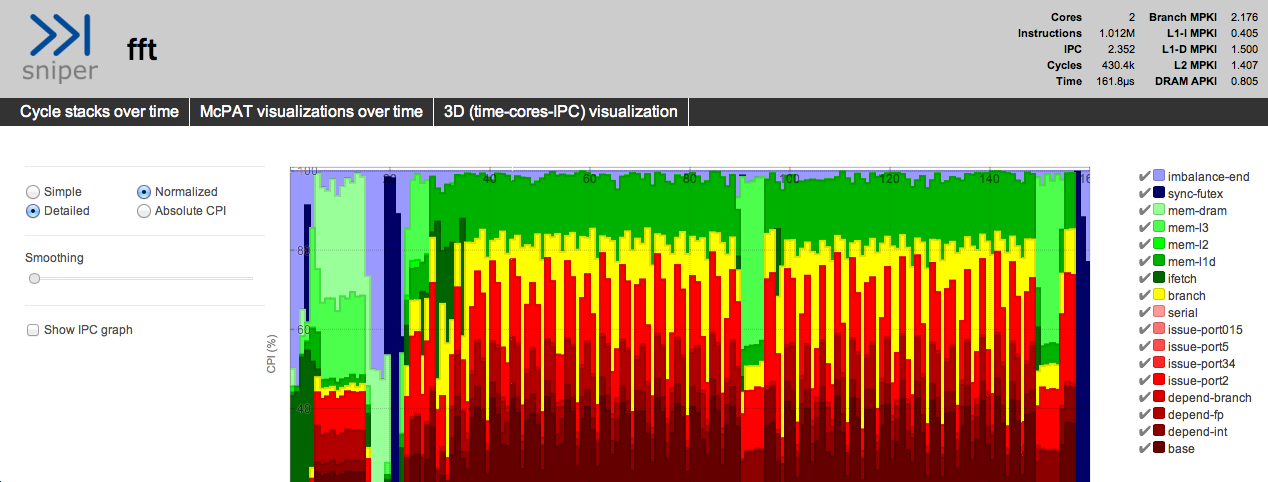
\includegraphics[width=1.0\linewidth]{fft-2-level2.png}
  \caption{
    \label{fig:fft-level2}
    CPI stack over time for Splash-2 FFT with 2 threads in the detailed, normalized view. The application was run in Sniper with the gainestown configuration in Sniper using the \cmd{--viz} and \cmd{--power} options.
}\end{figure}

The traditional CPI-stack (\cmd{sniper/tools/cpistack.py}) aggregates information from an entire run into a single stack.
This visualization (as seen in Figure~\ref{fig:fft-level2})
is an interactive graph of cycle stacks plotted over time. Two main options are provided.
The user can switch between a simple and a detailed view. In the simple view, the used cycles are grouped
in four main components: compute, branch, communicate and synchronize. The detailed view subdivides these
main components in more detailed components while keeping the colors of the main components the same. Components
that belong to the same main component have the same color with a different tint or shade. The second option provided
is the option to view a normalized or non-normalized cycle stack.
This visualization can be created by using the \cmd{--viz} option to the \cmd{run-sniper} command.

\subsubsection{McPAT visualizations plotted over time}
This visualization is similar to the cycle stacks plotted over time, instead showing the output
of McPAT over time. One can view the power and energy used during the different periods of execution of
the application. The user can switch between the visualization of power (W), energy (J) and energy (\%).
By default, the McPAT visualization is not generated because it can take quite a long time (many hours for long benchmarks).
We have recently updated McPAT to support CACTI caching both between and inside of runs. This has resulted in significant
performance improvements when running McPAT. Sniper versions after 4.1 have been enabled to automatically use the CACTI caching version
of McPAT on 64-bit hosts.
To generate the McPAT visualization in addition to the normal visualizations over time,
use the \cmd{--power} option in combination with the \cmd{--viz} option to \cmd{run-sniper}.

\subsubsection{3D Time-Cores-IPC visualization}

\begin{figure}\centering
  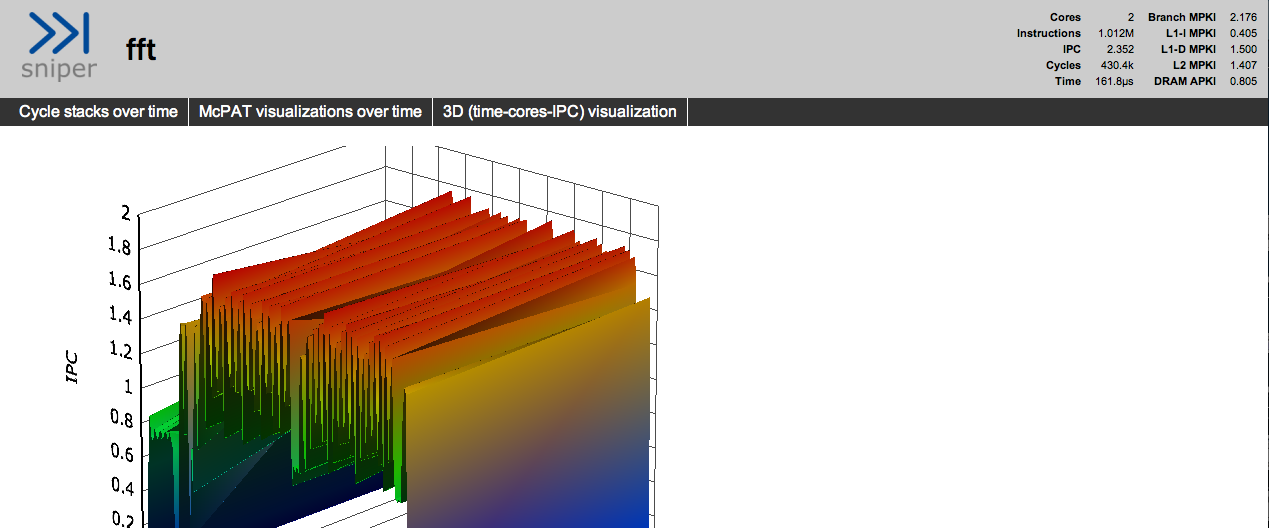
\includegraphics[width=1.0\linewidth]{fft-2-level3.png}
  \caption{
    \label{fig:fft-level3}
    CPI stack over time for Splash-2 FFT with 2 cores running with the gainestown configuration in Sniper.
}\end{figure}

As progress made on cores can be different, a higher-level overview of the IPC (instructions-per-cycle) for each core over time was added (Figure~\ref{fig:fft-level3}).
The result is a surface plot that indicates per-core IPC.
A low IPC can mean that an application is not making significant progress because of architectural or micro-architectural limitations.

\subsubsection{Topology}

\begin{figure}\centering
  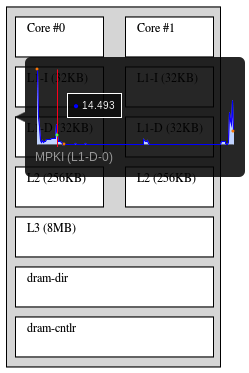
\includegraphics[width=.33\linewidth]{fft-2-topology.png}
  \caption{
    \label{fig:fft-topology}
    Topology of the gainestown microarchitecture with a sparkline showing the misses per 1000 instructions (MPKI) of the first L1 data cache.
    The sparkline shows the MPKI of the Splash-2 FFT application running on two cores.
}\end{figure}

Starting with Sniper version 4.2, the \cmd{--viz} option to \cmd{run-sniper} automatically generates the system topology as an additional section on the generated
web page. In addition to the topology information, with includes cache sizes and sharing configuration, the image is annotated with performance data.
Pop-ups display information about the different components: cores display their IPCs over time, caches display MPKI, and the DRAM controllers show APKI.

\subsubsection{Visualization notes}

\begin{itemize}
 \item The visualizations have been tested on Google Chrome version 23, Mozilla Firefox version 16 and Sarfari 6.02. Enable WebGL support in Safari to view the WebGL-optimized version of the 3D IPC plot.
 \item When the visualizations are not on a web server, Chrome will not render the visualizations correctly, although Firefox will.
 \item If the visualizations are slow, try to generate them with fewer, larger intervals.
 \item Generating the output for McPAT can take a lot of time if you are not using the CACTI-caching version. Note that the 32-bit versions compiled by us do not support caching.
\end{itemize}



\section{Command Listing}

\subsection{Main Commands}

\subsubsection{\cmd{run-sniper}}
\label{sec:cmd-run-sniper}

\cmd{run-sniper  [-n <ncores (1)>]  [-d <outputdir (.)>]  [-c <sniper-config>]  [-c [objname:]<name[.cfg]>,<name2[.cfg]>,...]  [-g <sniper-options>]  [-s <script>]  [--roi]  [--roi-script]  [--viz]  [--perf]  [--gdb]  [--gdb-wait]  [--gdb-quit]  [--appdebug]  [--appdebug-manual]  [--appdebug-enable]  [--power]  [--cache-only]  [--fast-forward]  [--no-cache-warming]  [--save-patch]  [--pin-stats]  [--mpi [--mpi-ranks=<ranks>] ]  \{--traces=<trace0>,<trace1>,... [--response-traces=<resptrace0>,<resptrace1>,...] | -- <cmdline>\}}

There are a number of ways to simulate applications inside of Sniper.  The traditional mode accepts a command line argument
of the application to run. Starting with Sniper 2.0, multiple single-threaded
workloads to be run on in Sniper via the SIFT feeder (\opt{--traces}).
Multiple multi-threaded applications can be run in Sniper as well via SIFT and the \opt{--response-traces} option starting with version 3.04.
This is automatically configured via the \opt{--benchmarks} parameter to \opt{run-sniper} in the integrated benchmarks suite.
In Sniper 4.0, single-node shared-memory MPI applications can now be run in Sniper.

\begin{itemize}[label=$$]
\item \opt{-n} --- Number of simulated cores (overrides the \opt{general/ncores} configuration option)
\item \opt{-d <dir>} --- Output directory for all generated files
\item \opt{-c <sniper-config>} --- Configuration file(s), see Section~\ref{configuration-files}
\item \opt{-c [objname:]<name[.cfg]>,<name2[.cfg]>,...} --- Setup a heterogeneous configuration for n items (cores by default) while setting the tag objnames to name, name2, etc.
\item \opt{-g <section/key=value>} --- Individual configuration setting(s), see Section~\ref{command-line-configuration}
\item \opt{-s <script>} --- Run script during the simulation, see Section~\ref{scripting}
\item \opt{--roi} --- Enable/disable detailed mode on SimRoiBegin()/SimRoiEnd() (default: whole program executed in detailed mode)
\item \opt{--roi-script} --- Allow ROI to be completely determined by script (start in fast-forward mode, ignore SimRoiBegin()/SimRoiEnd())
\item \opt{--viz} --- Generate visualizations, combine with \opt{--power} to enable McPAT runs. (default: output to viz/, Requires version 4.1+)
\item \opt{--perf} --- Run Sniper inside of the Linux 'perf stat' tool.
\item \opt{--gdb} --- Enable Pin tool debugging. Start executing the Pin tool right away
\item \opt{--gdb-wait} --- Enable Pin tool debugging. Halt when first attaching to the debugger
\item \opt{--gdb-quit} --- Enable Pin tool debugging. Automatically quit if no errors were detected
\item \opt{--appdebug} --- Enable Pin application debugging. Halt when first attaching to the debugger
\item \opt{--appdebug-manual} --- Enable Pin application debugging. Do not start gdb automatically, but allow the user to connect manually
\item \opt{--appdebug-enable} --- Enable Pin application debugging. Start executing the application right away
\item \opt{--power} --- Enable McPAT power runs. When used in combination with \opt{--viz}, also generate the McPAT output.
\item \opt{--cache-only} --- Only simulate caches during ROI
\item \opt{--fast-forward} --- Use fast-forwarding during the entire run
\item \opt{--no-cache-warming} --- Use fast-forward simulation before ROI (default is to use cache-only)
\item \opt{--save-patch} --- Save a patch (to \opt{sim.patch}) with the current Sniper code differences
\item \opt{--pin-stats} --- Enable basic pin statists. Normally saves to \opt{pin.log}
\item \opt{--mpi} --- Enable single-node (shared-memory) MPI simulation support. Works with MPICH2 and Intel MPI (Requires version 4.0+)
\item \opt{--mpi-ranks} --- Specify the number of ranks (if different from -n) (Requires version 4.0+)
\item \opt{--traces} --- Low-level SIFT interface. Specify a comma-separated list of SIFT input trace files. Normally, users will want to use the integrated benchmarks suite instead of using this interface directly (Requires version 2.0+).
\item \opt{--response-traces} --- Low-level SIFT interface. Specify a list of SIFT response trace pipes. Normally, users will want to use the integrated benchmarks suite instead of using this interface directly. (Requires version 3.04+)
\item \opt{<cmdline>} -- Application and options to simulate in Sniper
\end{itemize}



\subsection{Sniper Utilities}

\subsubsection{\cmd{tools/attachgdb.sh}}

\cmd{tools/attachgdb.py [-h|--help] [--all-threads] [--action=\{bt\}] [--abt] <pid>}

\begin{itemize}[label=$$]
\item \opt{--all-threads} --- Perform the action on all threads
\item \opt{--action=} --- Perform an action (default = bt, backtrace) on all threads
\item \opt{--abt} --- Shorthand for \cmd{attachgdb.py --all-threads --action=bt}
\end{itemize}

\subsubsection{\cmd{tools/cpistack.py}}

\cmd{tools/cpistack.py [-h (help)] [-d <resultsdir (default: .)>] [--partial <sec-begin>:<sec-end>] [-o <output-filename (cpi-stack)>] [--without-roi] [--simplified] [--no-collapse] [--no-simple-mem] [--time|--cpi|--abstime (default: time)] [--aggregate]}

\begin{itemize}[label=$$]
\item \opt{-d <dir>} --- Look into \opt{<dir>} to find the necessary files to compute a CPI-stack
\item \opt{--partial} --- Compute CPI stack over time span between specific statistics markers (default: \opt{roi-begin:roi-end})
\item \opt{-o <file>} --- Save gnuplot plotted data to <file>.png
\item \opt{--simplified} --- Create a CPI stack merging all items into the following categories: compute, communicate, synchronize
\item \opt{--no-collapse} --- Show all items, even if they are zero or below the threshold for merging them into the category other.
\item \opt{--time} --- Display CPI-stacks with execution time penalties instead of using CPI
\item \opt{--cpi} --- Display stacks with CPI data
\item \opt{--abstime} --- Normalize each thread's time to 1.0
\item \opt{--aggregate} --- Merge all CPI-stacks from multiple threads into a single CPI-stack
\end{itemize}


\subsubsection{\cmd{tools/mcpat.py}}

\cmd{tools/mcpat.py [-h (help)] [-d <resultsdir (default: .)>] [--partial <sec-begin>:<sec-end>] [-t <type: dynamic|rundynamic|static|total|area>] [-v <Vdd>] [-o <output-file (power{.png,.txt,.py})>}

\begin{itemize}[label=$$]
\item \opt{-d <dir>} --- Look into \opt{<dir>} to find the necessary files to compute a power stack
\item \opt{--partial} --- Compute power over time span between specific statistics markers (default: \opt{roi-begin:roi-end})
\item \opt{-o <file>} --- Save gnuplot plotted data to <file>.png
\item \opt{-t <type>} --- Output type of McPAT to plot: dynamic (dynamic power), rundynamic (runtime dynamic), static, total (dynamic + static), area
\item \opt{-v <vdd>} --- Override the process' default Vdd (V)
\end{itemize}


\subsection{SIFT Utilities}

\subsubsection{\cmd{record-trace}}

Record a SIFT instruction trace.

\cmd{./record-trace  -o <output file (default=trace)>  [-f <fast-forward instrs (default=none)] [-d <detailed instrs (default=all)] [-b <block size (instructions, default=all)> [--gdb|--gdb-wait|--gdb-quit] -- <cmdline>}

\begin{itemize}[label=$$]
\item \opt{-o <file>} --- Trace filename to create
\item \opt{-f <int>} --- Number of instructions to fast forward before starting to create the trace
\item \opt{-d <int>} --- Number of instructions to record in the trace
\item \opt{-b <int>} --- Block size.  By setting this value, multiple trace files will be created.  Filenames are names \cmd{<file>.<n>.sift} where \cmd{<file>} is set above (via \cmd{-o <file>}) and \cmd{n} is the block number.
\item \opt{<cmdline>} --- The command (and options) to run for trace collection
\end{itemize}

\subsubsection{\cmd{sift/siftdump}}

Review the contents of a SIFT trace.

\cmd{./siftdump <file1.sift> [<fileN.sift> ...]}

\begin{itemize}[label=$$]
\item \opt{<file>} --- One or more SIFT trace files to view
\end{itemize}

\subsection{Visualization}

\subsubsection{\cmd{tools/viz.py}}
Generate the visualizations.

\cmd{tools/viz.py [-h|--help (help)] [-d <resultsdir (default: .)>] [-t <title>] [-n <num-intervals (default: all$\_$intervals)>] [-i <interval (default: smallest$\_$interval)>] [-o <outputdir>] [--mcpat] [-v|--verbose]}

\begin{itemize}[label=$$]
\item \opt{-d <resultsdir>} --- Look into \opt{<resultsdir>} to find the necessary files to generate the visualizations
\item \opt{-t <title>} --- Name of the application, will be used as title of the visualization
\item \opt{-n <num-intervals>} --- The visualization will be generated for \opt{<num-intervals>} intervals
\item \opt{-i <interval>} --- The used interval size will be \opt{<interval>} 
\item \opt{-o <outputdir>} --- Save the result to \opt{<outputdir>}
\item \opt{--mcpat} --- Generate visualizations for McPAT
\item \opt{-v|--verbose} --- Verbose output
\end{itemize}

\subsubsection{\cmd{tools/viz/level2.py}}
Generate the visualization of the cycle stacks over time.

\cmd{tools/viz/level2.py [-h|--help (help)] [-d <resultsdir (default: .)>] [-t <title>] [-n <num-intervals (default: all$\_$intervals)>] [-i <interval (default: smallest$\_$interval)>] [-o <outputdir>] [--mcpat] [-v|--verbose]}

\begin{itemize}[label=$$]
\item \opt{-d <resultsdir>} --- Look into \opt{<resultsdir>} to find the necessary files to generate the visualizations
\item \opt{-t <title>} --- Name of the application, will be used as title of the visualization
\item \opt{-n <num-intervals>} --- The visualization will be generated for \opt{<num-intervals>} intervals
\item \opt{-i <interval>} --- The used interval size will be \opt{<interval>}
\item \opt{-o <outputdir>} --- Save the result to \opt{<outputdir>}
\item \opt{--mcpat} --- Generate visualizations for McPAT
\item \opt{-v|--verbose} --- Verbose output
\end{itemize}

\subsubsection{\cmd{tools/viz/level3.py}}
Generate the 3D Time-Cores-IPC visualization.

\cmd{tools/viz/level3.py [-h|--help (help)] [-d <resultsdir (default: .)>] [-t <title>] [-n <num-intervals (default: all$\_$intervals)>] [-i <interval (default: smallest$\_$interval)>] [-o <outputdir>] [-v|--verbose]}

\begin{itemize}[label=$$]
\item \opt{-d <resultsdir>} --- Look into \opt{<resultsdir>} to find the necessary files to generate the visualizations
\item \opt{-t <title>} --- Name of the application, will be used as title of the visualization
\item \opt{-n <num-intervals>} --- The visualization will be generated for \opt{<num-intervals>} intervals
\item \opt{-i <interval>} --- The used interval size will be \opt{<interval>}
\item \opt{-o <outputdir>} --- Save the result to \opt{<outputdir>}
\item \opt{-v|--verbose} --- Verbose output
\end{itemize}



\section{Comprehensive Option List}

\subsection{Base Sniper Options}
\lstinputlisting[caption=Base options (base.cfg),rulecolor=\color{DarkSlateBlue},language=ini]{../../config/base.cfg}

\subsection{Options used to configure the Nehalem core}
\lstinputlisting[caption=Nehalem options (nehalem.cfg),rulecolor=\color{DarkSlateBlue},language=ini]{../../config/nehalem.cfg}

\subsection{Options used to configure the Gainestown processor}
\lstinputlisting[caption=Gainestown options (gainestown.cfg),rulecolor=\color{DarkSlateBlue},language=ini]{../../config/gainestown.cfg}

\subsection{Sniper Prefetcher Options}
\lstinputlisting[caption=Prefetcher options (prefetcher.cfg),rulecolor=\color{DarkSlateBlue},language=ini]{../../config/prefetcher.cfg}

\subsection{DRAM Cache Options}
\lstinputlisting[caption=DRAM cache options (dram-cache.cfg),rulecolor=\color{DarkSlateBlue},language=ini]{../../config/dram-cache.cfg}


\subsection{SimAPI Commands}
\label{sec:option-simapi}

\lstinputlisting[caption=SimAPI,rulecolor=\color{DarkSlateBlue},language=C]{sim_api_doc.h}

%%\subsection{Sniper Configuration Options}

\ignore{
\section{Todo}

Some high-level remarks, needs to be integrated.

\subsection{Sniper use cases}

\subsubsection{Architectural exploration}

\begin{itemize}
\item High-level architecture design (number of cores, core types)
\item Cache studies: topology, capacity, bandwidth. Since Sniper models the memory hierarchy
      in reasonable detail, replacement policies or coherence algorithms can also be studied.
\item Heterogeneity studies: big versus small cores, big {\em and} small cores, on-chip frequency variations,
      hardware (and software) thread scheduling and migration to manage all of this
\end{itemize}

\subsubsection{Software \& compiler optimization}

\begin{itemize}
\item Since Sniper is fast enough to run reasonable-sized workloads on future or
      hypothetical machines, you can tune algorithms for cache size, or test the effect
      of compiler optimizations or software prefetching when taking into account changes
      in pipeline depth, instruction latencies and issue limitations, cache sizes and latencies, etc.
\item Parallelization, vectorization, study scaling to larger core counts (excluding effects caused
      by OS limitations, and assuming new (vector or other) instructions can be emulated)
\item Future \& hypothetical machines: see what happens to your algorithm/compiler optimization
      when machines grow larger (or cores become more simple?). Or: what hardware would be required
      to support this type of software algorithm / optimization?
\item Feedback: on-line CPI stacks allow your application to learn about how efficiently it's running.
      Auto-tuners, adaptive algorithms.
\end{itemize}

\subsubsection{Co-design}

Of course it's possible to combine these two and co-optimize algorithm, implementation, compiler and hardware all at the same time.


\subsection{Non-use cases}

\begin{itemize}
\item Workloads where significant OS involvement is expected (commercial applications,
      maybe managed languages), or when scaling is restrained by OS limitations
\item Low-level architecture optimization. Sniper assumes that a processor design is balanced, meaning that application performance is largely determined by a few key architectural components, the others are not modeled. When simulating an existing architecture this assumption is usually valid, as great care is taken by real processor designers to balance the architecture. Similarly, when doing high-level hardware exploration studies that are to determine the best trade-offs for high-level architectural characteristics such as issue widths, core counts and cache sizes; one should assume that later on, a further design phase will follow in which the design is balanced out by sizing lower-level structures such as load-store queues to match. (For this reason, modeling too much detail in higher-level studies is both unneeded and unwanted: one wouldn't want to write off a potential architecture early on because of a perceived limitation in the size of its rename registers, as such a defect would easily have been solved in a later design stage. Therefore, modeling should be restricted to those hardware characteristics which have a large impact on performance and/or are important to pin down early on).
\end{itemize}



\subsection{Hardware validation}

We do not aim to achieve great accuracy compared to real hardware. For
one, the specific parameters and characteristics of current-day
machine with which we can compare are not necessarily representative
for the future machines we aim to model. Secondly, we aim to provide a
high-level insight into what architectural and algorithmic
enhancements affect performance and energy consumption, and how these
can be traded off against each other. Here also, low-level
implementation details detract from the insight that could be gained,
rather than improve accuracy of the end result. Therefore, hardware
validation must be seen as a way of debugging and gaining confidence
into the simulation models, making sure that those components that
matter are modeled correctly and to a sufficient level of detail ---
rather than being an end goal in itself.
}


\end{document}
